\section{Introduction}

\begin{figure}[b]
	\begin{minipage}[c]{0.5\textwidth}
		\begin{center}
		\centerline{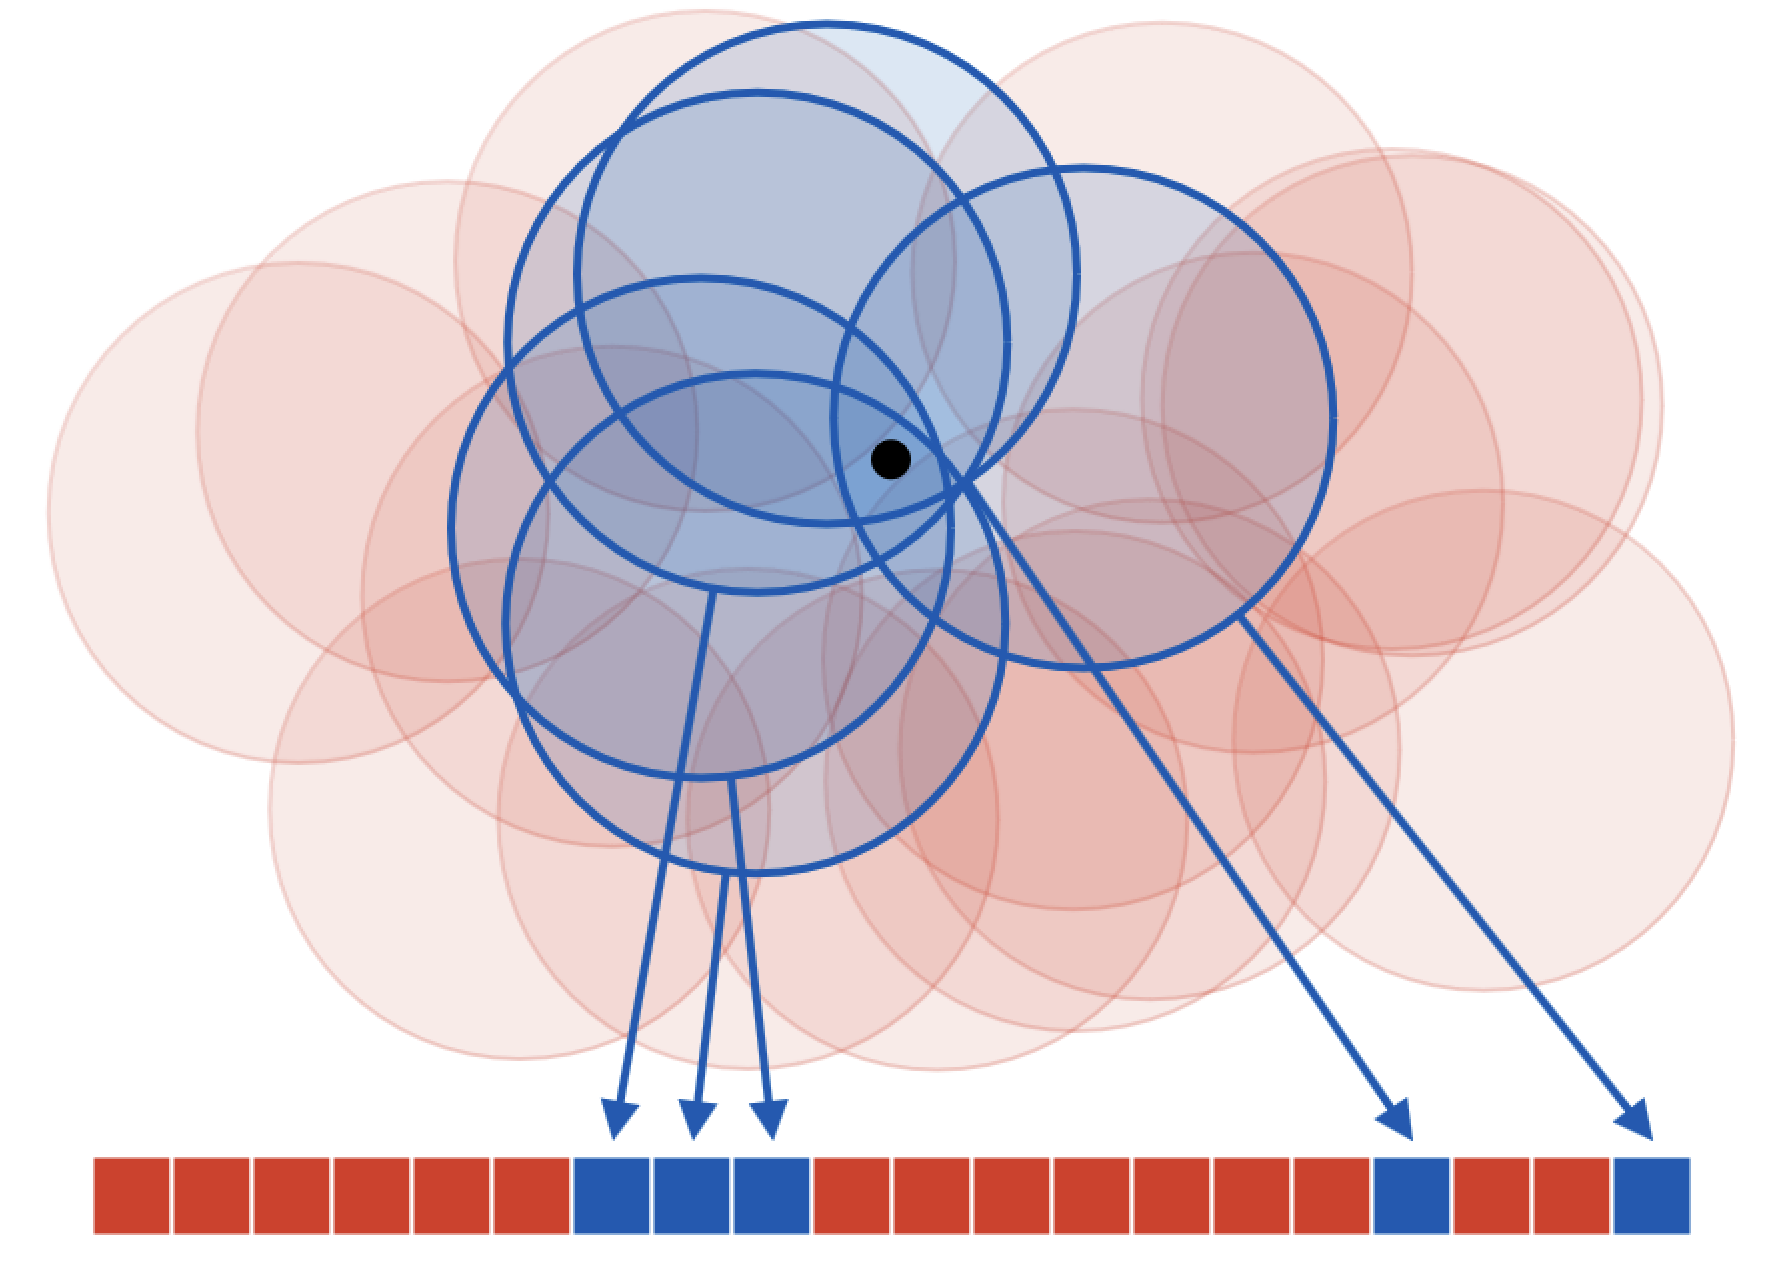
\includegraphics[width=0.8\textwidth]{../figures/coarse_code_short.png}}
				\end{center}
	\end{minipage}%
	\begin{minipage}[c]{0.5\textwidth}
		\vspace{-20pt}
		\caption{A coarse code representing a point on a plane. Each ``neuron,'' drawn as a red or blue square, encodes whether the point belongs to an associated ``receptive field.'' Although no neuron gives specific information on the position of the point, the overall code determines its position with reasonable accuracy.}
		\label{coarse-code}
	\end{minipage}
\end{figure}

If each neuron in a given neural network coded for a ``meaningful'' feature of its input, we could hope to reverse-engineer this network's overall behavior on a neuron-by-neuron basis. However, individual neurons of real-world networks often lack clear interpretations. For example, both language models and vision models have been found to learn neurons that correlate simultaneously with apparently unrelated features. (See for example \citet{nguyen_multifaceted_2016}, \citet{zhang_sample_2023} and \citet{olah_zoom_2020}.)

The difficulty of interpreting a network in terms of its local activity---and in particular, the appearance of so-called ``polysemantic neurons''---is not surprising from a connectionist viewpoint. Since at least the 1980s, proponents of neural networks have argued that these systems may naturally use \textbf{distributed representations}---coding schemes where individual features are represented by patterns spread over many neurons, and conversely where each neuron carries information on many features. (This term was apparently coined in \cite{rumelhart_parallel_1986}, Chapter 3.) In contrast, a \textit{local} representation would dedicate each neuron to a single feature. See \cite{thorpe_local_1989} for a general discussion of local and distributed codes. \Cref{coarse-code} illustrates a classic example of a coarse code, one kind of distributed representation.

As of now, relatively little is known about how deep neural networks learn to represent information in their hidden layers or to what extent this information can be interpreted. However, should ``interpretable features'' exist, the connectivist viewpoint makes it natural that they would typically be stored with non-local codes. This is a common assumption in interpretability research today; for example, when \citet{meng_locating_2022} intervened on an MLP layer of a language model to ``edit'' a factual association, both the ``subject'' and the ``fact'' were modeled as vectors of neuron activations rather than as individual neurons.

How can we infer latent features learned by a neural network? One simple proposal is to model an activation vector $x$ as a linear projection
\begin{equation*}
	x = F y \label{eq:linear-model}
\end{equation*}
of some high-dimensional and \textit{sparse} vector $y$ of latent features. We refer to the columns of $F$ as codewords and the whole matrix $F$ as a dictionary. Since $x$ is a linear superposition of codewords, we will call it a \textbf{superposition code} for $y.$ It is a remarkable fact that, for certain matrices $F,$ the linear projection $x = F y$ can code uniquely for a sparse vector $y$ even when the dimension of $x$ is (much) smaller than the dimension of $y.$ The task of inferring the sparse vector from its linear projection is known as sparse reconstruction, and the task of inferring the dictionary $F$ from a distribution over $x$ is called dictionary learning. Both of these problems have been studied in the field of compressive sensing, although with different applications in mind. (See \cite{elad_sparse_2010} for a review of classic work in the context of signal and image processing.)

Already in 2015, \cite{faruqui_sparse_2015} used a dictionary learning method to derive sparse latent codes for word embeddings and argued that these latents were more interpretable than the original embedding dimensions. More recently, a series of works beginning with \cite{yun_transformer_2021} have applied dictionary learning to the internal representations of transformer-based language models. \cite{cunningham_sparse_2023} suggested the use of \textbf{sparse autoencoders} (SAEs) and \cite{templeton_scaling_2024, gao_scaling_2024} scaled sparse autoencoders to production-size large language models.

To infer a latent representation $y \in \R^N$ from an activation vector $x \in \R^d,$ sparse autoencoders use an estimate like $\hat y(x) = \sigma(G x)$ for some learnable matrix $G \colon \R^{N \times d}$ and some simple non-linear thresholding function $\sigma.$ Given a latent vector $\hat y,$ the In \cite{gao_scaling_2024}, the number of latent dimensions considered was on the order of $N = 10^{6}$ and latent representations $y$ were assumed to have on the order of $k = 10^{2}$ non-zero coefficients.

\cite{templeton_scaling_2024} showed that latent features learned by SAEs are often highly intepretable, and that intervention on these features allows ``steering'' language models in predictable ways. However, as reported in \cite{gao_scaling_2024}, even SAEs with extremely large numbers of latents suffer from an apparently irreducible reconstruction error. According to \cite{sharkey_open_2025}, understanding the limitations of SAEs---and dictionary learning in general---is an important open question in the research program of mechanistic interpretability.

\subsection*{Contributions}

Over the course of computation, it is common for programs to use more memory than was required to store their input data. Similarly, it is natural to expect that the entropy of a ``simple'' (or ``interpretable'') description for the residual vectors within a language model is not bounded by the entropy of language. Methods like sparse autoencoders look to provide descriptions of these hidden activations, but very little is known about what kind of information is being carrier. One basic and natural question is \textit{how much} information can hypothetically be stored in an activation vector.

In many classical situations, this question is answered by well-known ideas from information theory. Given a ``channel'' with certain characteristics---for example, a band-limited telephone connection or a binary storage device with a certain failure rate---the amount of information we can effectively transmit is asymptotically characterized by a ``channel capacity'' measured in bits per unit of channel usage. The goal of this paper is to study the carrying capacity of sparse superposition codes in a regime that is applicable to sparse autoencoders. Our analysis focuses on a toy example, described in more detail in \Cref{sec:codes}. Our main findings are the following.

First, in an asymptotic regime of sublinear sparsity ($\ln k \le \eta \ln N$ for some $\eta < 1$), very simple ``one-step methods'' can reliably decode superposition codes when $d$ is a constant factor greater than the Shannon limit. Our asymptotic results agree very well with numerical experiments, providing good ``rules of thumb'' in practice for the top-$k$ decoder.

On the other hand, we also show that the constant factor grows to infinity as $\eta$ goes to $1,$ and can already be surprisingly large for values of $(N, k)$ typical for sparse autoencoders. [continue]

\begin{figure}
	\begin{center}
	\begin{minipage}[]{0.63\textwidth}
		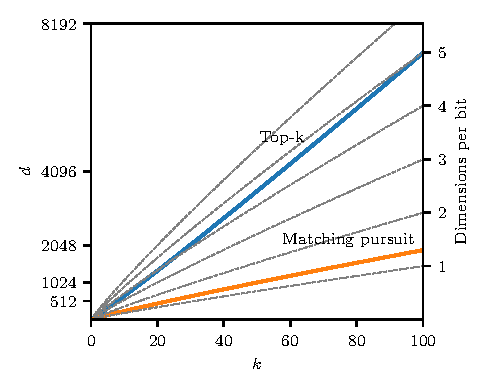
\includegraphics[width=0.95\textwidth]{../figures/storyline}
	\end{minipage}%
	\begin{minipage}[]{0.37\textwidth}
		\vspace{-29pt}\caption{An overview of the minimum codeword dimension $d$ required for two different methods to reliably decode a uniformly chosen $k$-sparse subset of $\{1, \dots, 2^{20} \}$ from a superposition of codewords from an i.i.d.\ Rademacher dictionary. The inverse ``bitrate'' $d/H(k),$ where $H(k) = \log_2 \binom N k \approx k \log_2(e N/k),$ is indicated by the right axis. Top-$k$ is a method currently used by sparse autoencoders, and matching pursuit is a relatively cheap iterative algorithm.}
		\label{fig:storyline}
	\end{minipage}
	\end{center}
\end{figure}

How ``efficient,'' in terms of bitrate, are the codes used by real neural networks? Of course, it would not make sense for a network to use a code that requires a costly iterative decoding process before it can be used. However, the success of matching pursuit suggests that neural networks may be able to improve over the bitrates of one-step estimates while paying a relatively small computational price. Although our analysis is restricted to a toy scenario, we hope these results inform future work on modeling distributed representations.

\subsection*{Related Work}

Recently, various authors have studied the underperformance of SAEs and proposed ways to improve these methods. For example, \cite{rajamanoharan_improving_2024} proposed \textit{gated SAEs} to mitigate ``feature shrinkage,'' and \cite{bussmann_learning_2025} proposed \textit{Matryoska SAEs} to deal with problems related to ``feature absorption.''

Especially relevant to this work is the proposal of \textit{inference-time optimization} (ITO), which involves replacing the encoder of an SAE with an iterative optimization method at inference time---that is, after the dictionary $F$ has already been learned. For example,  \cite{engels_decomposing_2024} evaluated gradient pursuit as an inference-time optimization method. However, if the restrictive encoders used by SAEs at training time cannot discern read certain attributes of the sparse latent signal, then the corresponding codewords will not appear in the learned dictionary. This may explain the limited improvements attained so far by ITO. We hope the present work helps clarify these questions, especially for readers who may not be familiar with ideas from compressive sensing.
